%%\documentclass[a4paper, 12pt]{scrreprt}

\documentclass[a4paper, 12pt]{scrartcl}
%usepackage[german]{babel}
\usepackage{microtype}
%\usepackage{amsmath}
%usepackage{color}
\usepackage[utf8]{inputenc}
\usepackage[T1]{fontenc}
\usepackage{wrapfig}
\usepackage{lipsum}% Dummy-Text
\usepackage{multicol}
\usepackage{alltt}
%%%%%%%%%%%%bis hierhin alle nötigen userpackage
\usepackage{tabularx}
\usepackage[utf8]{inputenc}
\usepackage{amsmath}
\usepackage{amsfonts}
\usepackage{amssymb}

%\usepackage{wrapfig}
\usepackage[ngerman]{babel}
\usepackage[left=25mm,top=25mm,right=25mm,bottom=25mm]{geometry}
%\usepackage{floatrow}
\setlength{\parindent}{0em}
\usepackage[font=footnotesize,labelfont=bf]{caption}
\numberwithin{figure}{section}
\numberwithin{table}{section}
\usepackage{subcaption}
\usepackage{float}
\usepackage{url}
%\usepackage{fancyhdr}
\usepackage{array}
\usepackage{geometry}
%\usepackage[nottoc,numbib]{tocbibind}
\usepackage[pdfpagelabels=true]{hyperref}
\usepackage[font=footnotesize,labelfont=bf]{caption}
\usepackage[T1]{fontenc}
\usepackage {palatino}
%\usepackage[numbers,super]{natbib}
%\usepackage{textcomp}
\usepackage[version=4]{mhchem}
\usepackage{subcaption}
\captionsetup{format=plain}
\usepackage[nomessages]{fp}
\usepackage{siunitx}
\sisetup{exponent-product = \cdot, output-product = \cdot}
\usepackage{hyperref}
\usepackage{longtable}
\newcolumntype{L}[1]{>{\raggedright\arraybackslash}p{#1}} % linksbündig mit Breitenangabe
\newcolumntype{C}[1]{>{\centering\arraybackslash}p{#1}} % zentriert mit Breitenangabe
\newcolumntype{R}[1]{>{\raggedleft\arraybackslash}p{#1}} % rechtsbündig mit Breitenangabe
\usepackage{booktabs}
\renewcommand*{\doublerulesep}{1ex}
\usepackage{graphicx}
\usepackage{chemformula}



%\begin{document}
\setlength\abovedisplayshortskip{20pt}
\setlength\belowdisplayshortskip{20pt}
\setlength\abovedisplayskip{20pt}
\setlength\belowdisplayskip{20pt}
\section {Auswertung}
Um eine Relation zwischen Leitfähigkeit und Konzentration des Produktes zu erhalten, wurde eine Eichgerade durch die lineare Regression der Kalibrierungsmessreihe bestimmt (vgl. Abbildung \ref{Eichgerade}). Ferner wurde die Konzentration der Urease im Prozess als Konstant angenommen ($ 78\,[\si{\mu S/cm}]$) und von jeder Messung subtrahiert, um aus der vorliegenden Leitfähigkeit die Produktkonzentration gemäß folgender Gleichung abzuleiten : \\
\\
Sei : \\
 $[$P$]_M$ die Konzentration des Produktes in einer Messung\\
 $\sigma_M$ die gemessene Leitfähigkeit in $[\si{\mu S/cm}]$\\
  $\sigma_U$ die konstante Leitfähigkeit der Urease bei gegebener Verdünnung \\
  $f()$ die Eichfunktion, die eine Leitfähigkeit in die Produktkonzentration abbildet.\\
  \\
  Es gilt :
\begin{equation}
[\text{P}]  \sim \sigma_M \quad| \quad [\text{P}]=f(\sigma_M-\sigma_U)
\label{Eichgleichung}
\end{equation}
\begin{figure}[H]
	\centering	
	\begin{minipage}{1\textwidth}
		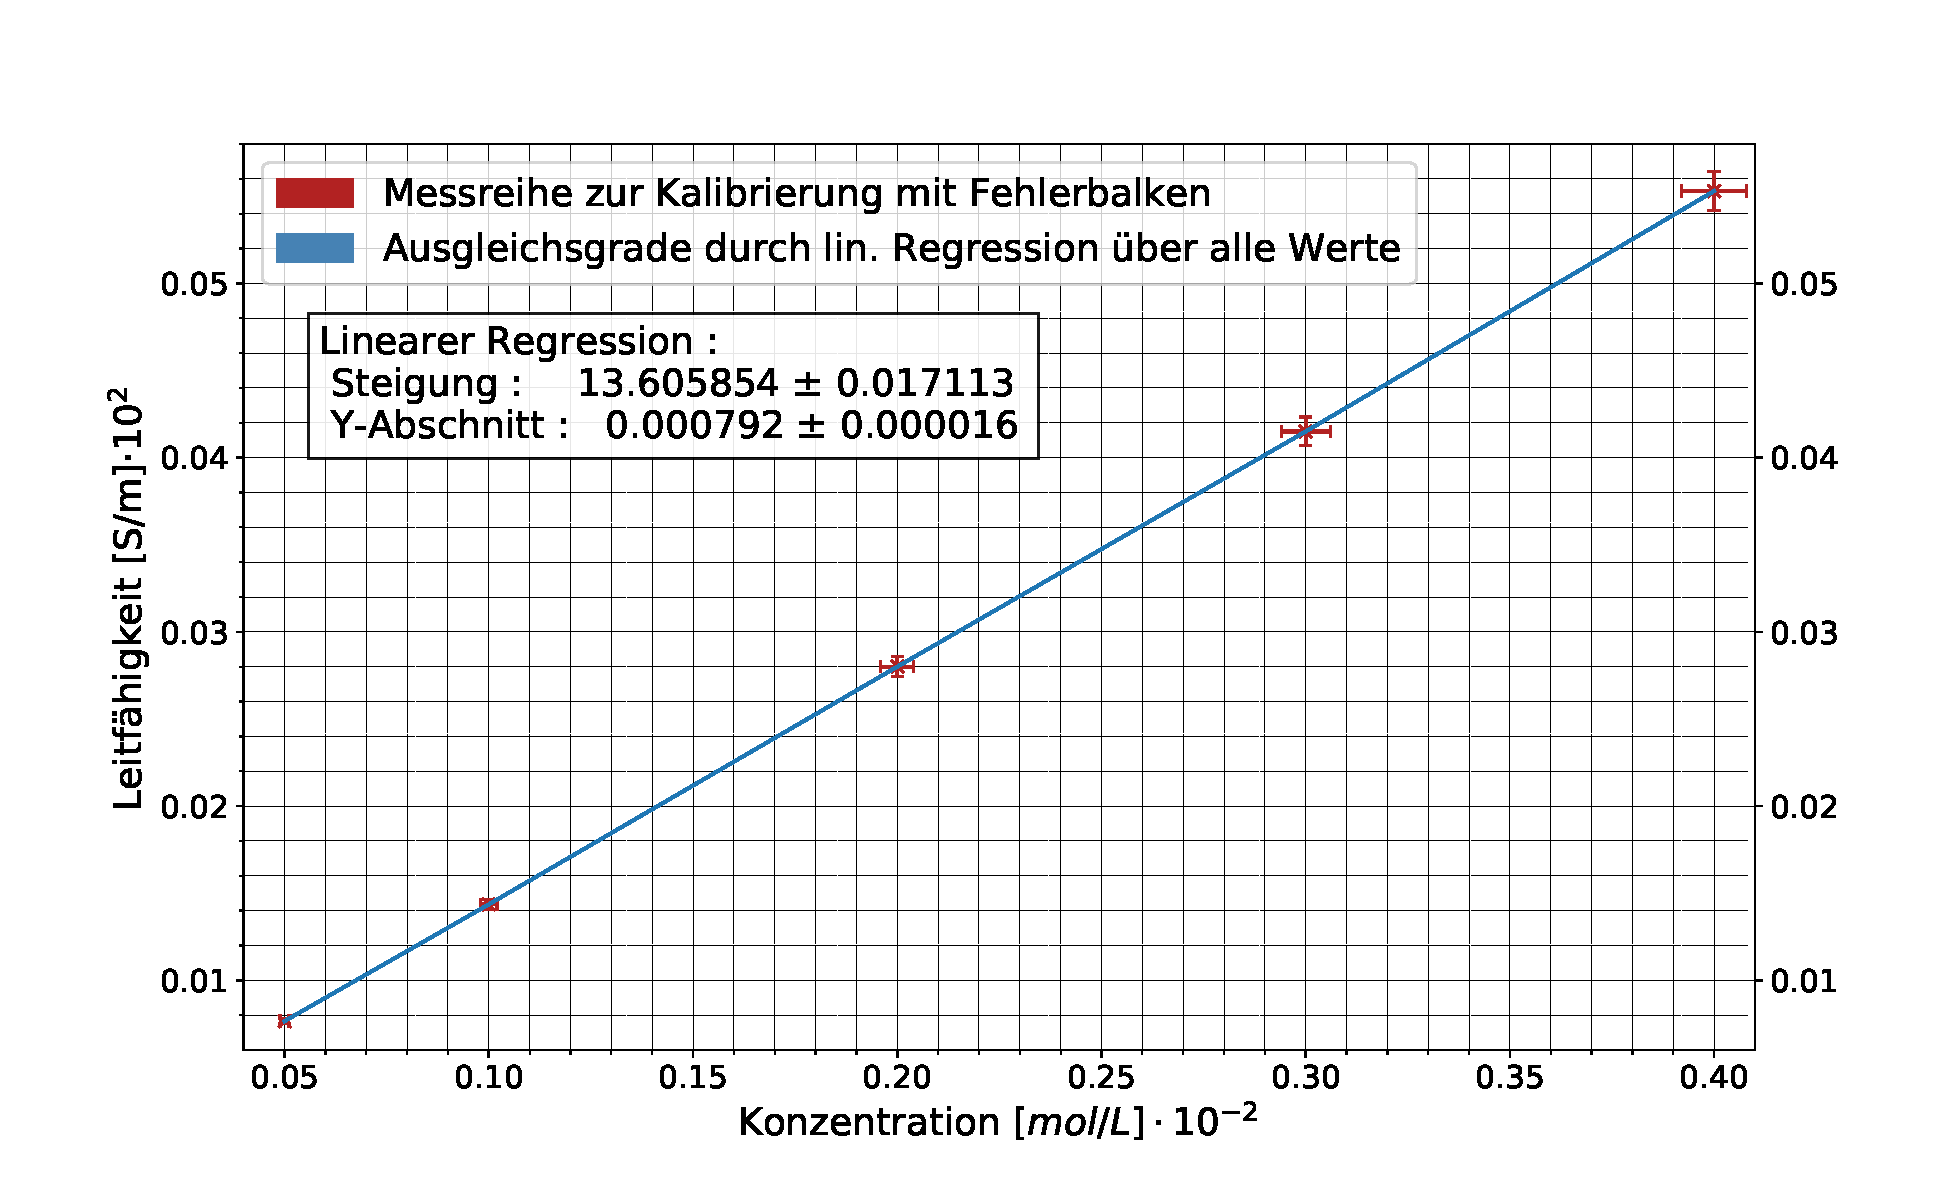
\includegraphics[width=\columnwidth]{Bilder/Kalibierung.pdf}
	\end{minipage}
	\caption{Eichgerade mithilfe der lineare Regression der Kalibrierungsreihe durch eine Routine in der Programmiersprache \textit{python}. Fehlerbalken resultieren aus Messungenauigkeit sowie Abmessungsfehler sowie dem Fehler des Verfahrens.}
	\label{Eichgerade}
\end{figure}
Im folgenden Schritt wurden die neun durchgeführten Messreihen in einer Abbildung als zeitliche Messung der Konzentration aufgetragen. Insbesondere wurde hierfür Gleichung \ref{Eichgleichung} verwendet um aus der eigentlich gemessene Leitfähigkeit die Konzentration zu bestimmen. Der Fehler ergibt sich hier als Fehler des Verfahrens sowie als Fehler basierend auf der fehlerbehaftete Eichfunktion.
\begin{figure}[H]
	\centering	
	\begin{minipage}{1\textwidth}
		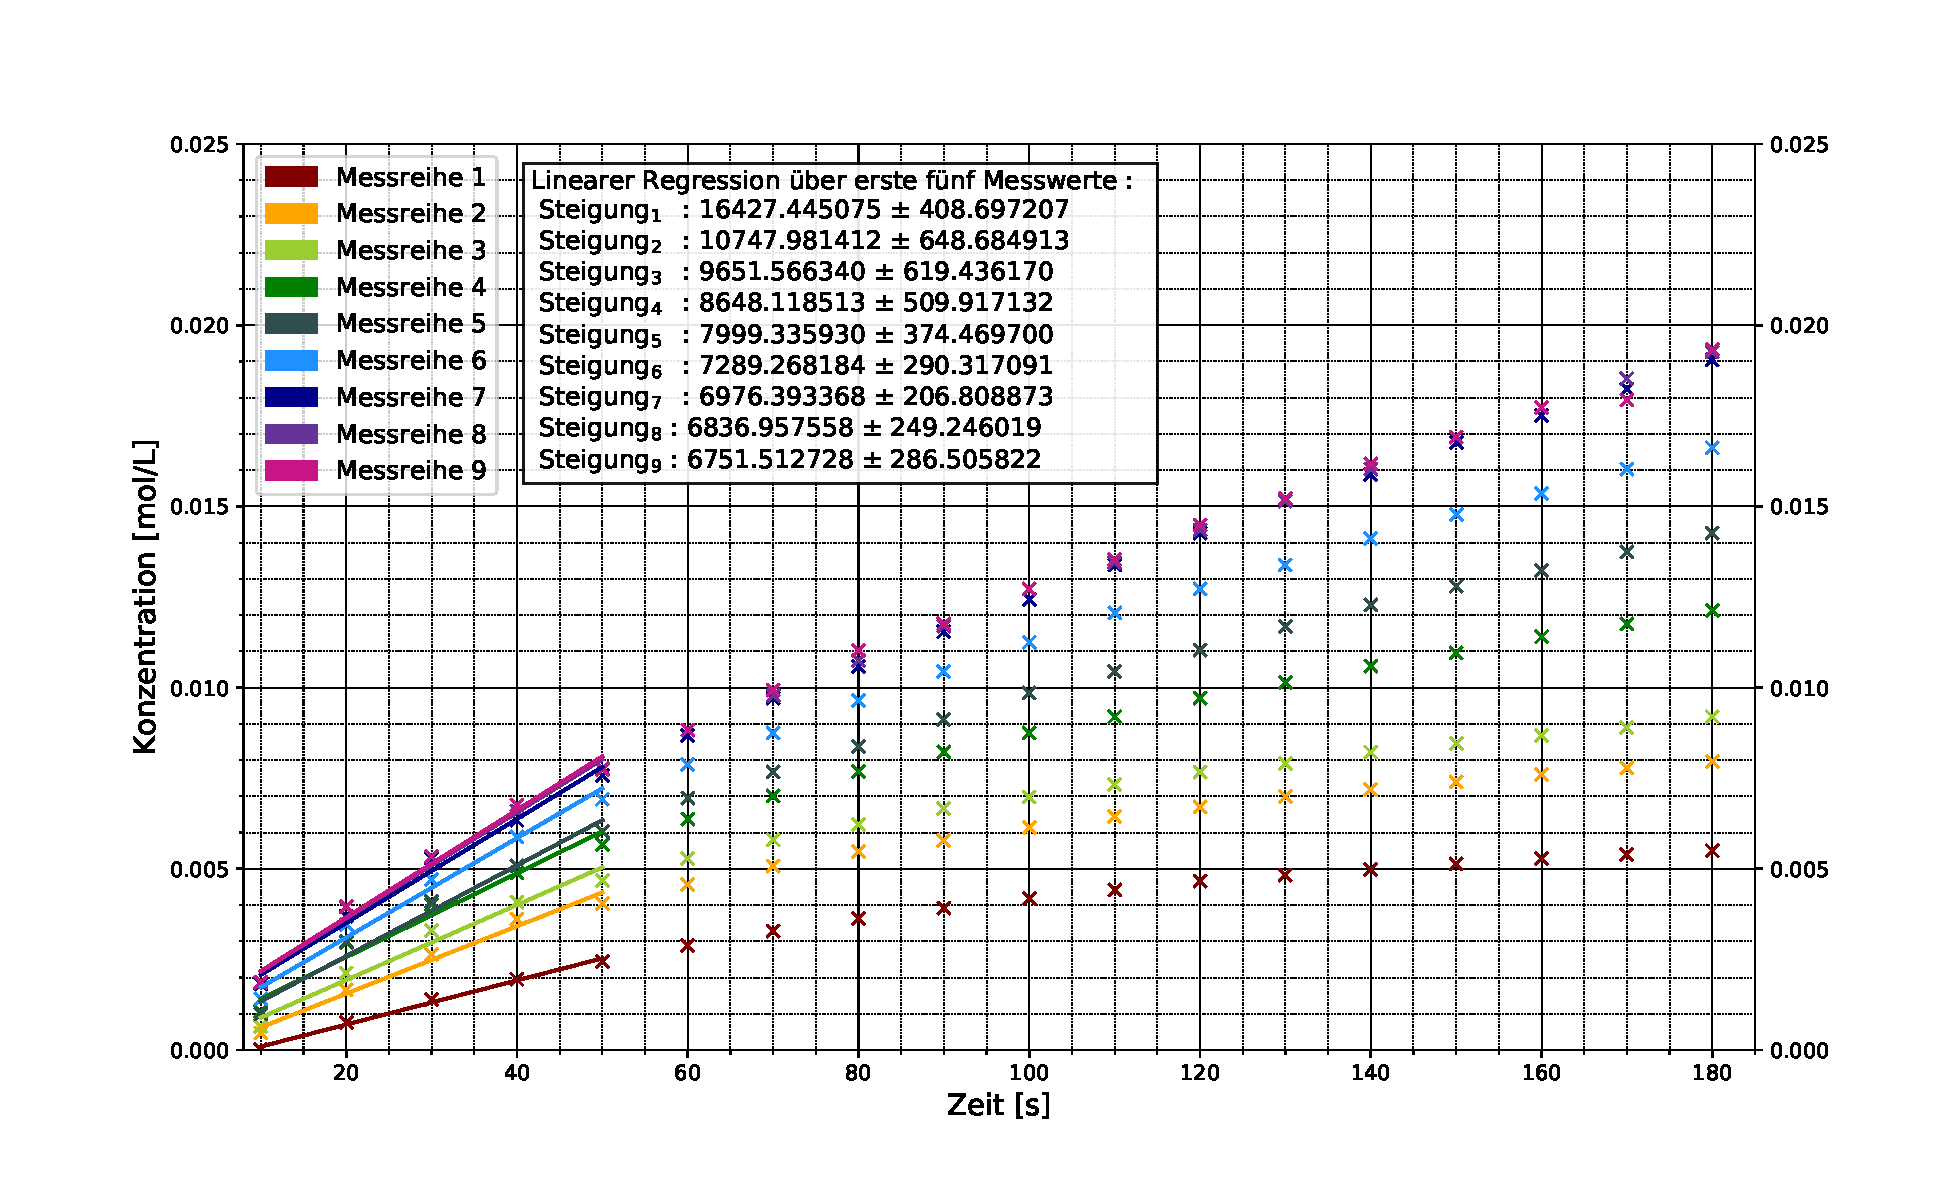
\includegraphics[width=\columnwidth]{Bilder/Messreihe.pdf}
	\end{minipage}
	\caption{Auftragung der neun durchgeführte Messreihen der Konzentration über der Zeit. Die Ausgleichsgeraden im Bereich der ersten fünf Messpunkte wurde durch eine lineare Regression in der Programmiersprache \textit{python} erzeugt, ferner die Steigung dieser Geraden ermittelt sowie dessen Fehler.}
	\label{Messreihe}
\end{figure}
Wichtig ist hier, dass die betreffenden Steigungen sich auf die Konzentrationszunahme der gemessenen Leitfähigkeit, also der Ammoniumcarbonatkonzentration bezieht. Die erhaltenen Steigungen bezogen auf die verwendete Verdünnung sowie der zugehörigen Fehler wurden in folgender Tabelle in signifikanten Stellen angegeben.
\begin{table}[H]
\centering
\label{Steigungstabelle}
	\caption{Steigungen der Ausgleichsgraden, welche durch eine lineare Regression der ersten fünf Messwerte erhalten wurden. Die lineare Regression erfolte über eine Routine in \textit{python}}
	\begin{tabular}{C{0.15\linewidth}|C{0.15\linewidth}C{0.25\linewidth}C{0.3\linewidth}}
		Messreihe  &  Steigung $\left[\si{\frac{s\cdot mol}{L}}\right] \cdot 10^{-3}$ &  Absoluter Fehler $\left[\si{\frac{s \cdot mol}{L}}\right] \cdot 10^{-3}$ & Konzentration Harnstoff $\left[\si{mol/L}\right]\cdot 10^{-2}$ \\
		\hline \addlinespace[1ex] 
		$ 1$ & $1.120$ & $\pm 0.025$ & 0.05\\
		$2$ & $1.684$& $ \pm 0.089$ &0.10\\
		$3$ & $1.856$& $\pm 0.098$ &0.15\\
		$4$ &$2.061$& $\pm 0.095$&0.2\\
		$5$&  $2.248$&  $\pm 0.082$ &0.3\\
		$6$&  $2.490$&  $\pm 0.082$&0.4\\
		$7$ &  $2.619$&$\pm 0.066$&0.6\\
		$8$ & $2.664$&$\pm  0.082$ &0.8\\
		$9$ &  $2.697$& $\pm 0.099$ &1\\
	\end{tabular}
\end{table}
Mithilfe dieser wurde ein \textit{Lineweaver-Burk-Plot} angefertigt um die gesuchten Größen $v_{max}\, , \, K_M\, ,\, k_2$ aus den bestimmten Steigungen, also Anfangsgeschwindigkeiten $v_0$, zu bestimmen. Hierfür wurde insbesondere Gleichung \ref{eq:Grenzfall} verwendet, also die Annahme eines linearen Verlaufs der somit formalen Reaktion nullter Ordnung, für die ersten Messwerte einer jeden gezeigten Messreihe in Abbildung \ref{Messreihe}. Die ermittelten Anfangsgeschwindigkeit wurden über die zugehörige Konzentration des Harnstoffs in einem reziproken Raum aufgetragen.
\begin{figure}[H]
	\centering	
	\begin{minipage}{1\textwidth}
		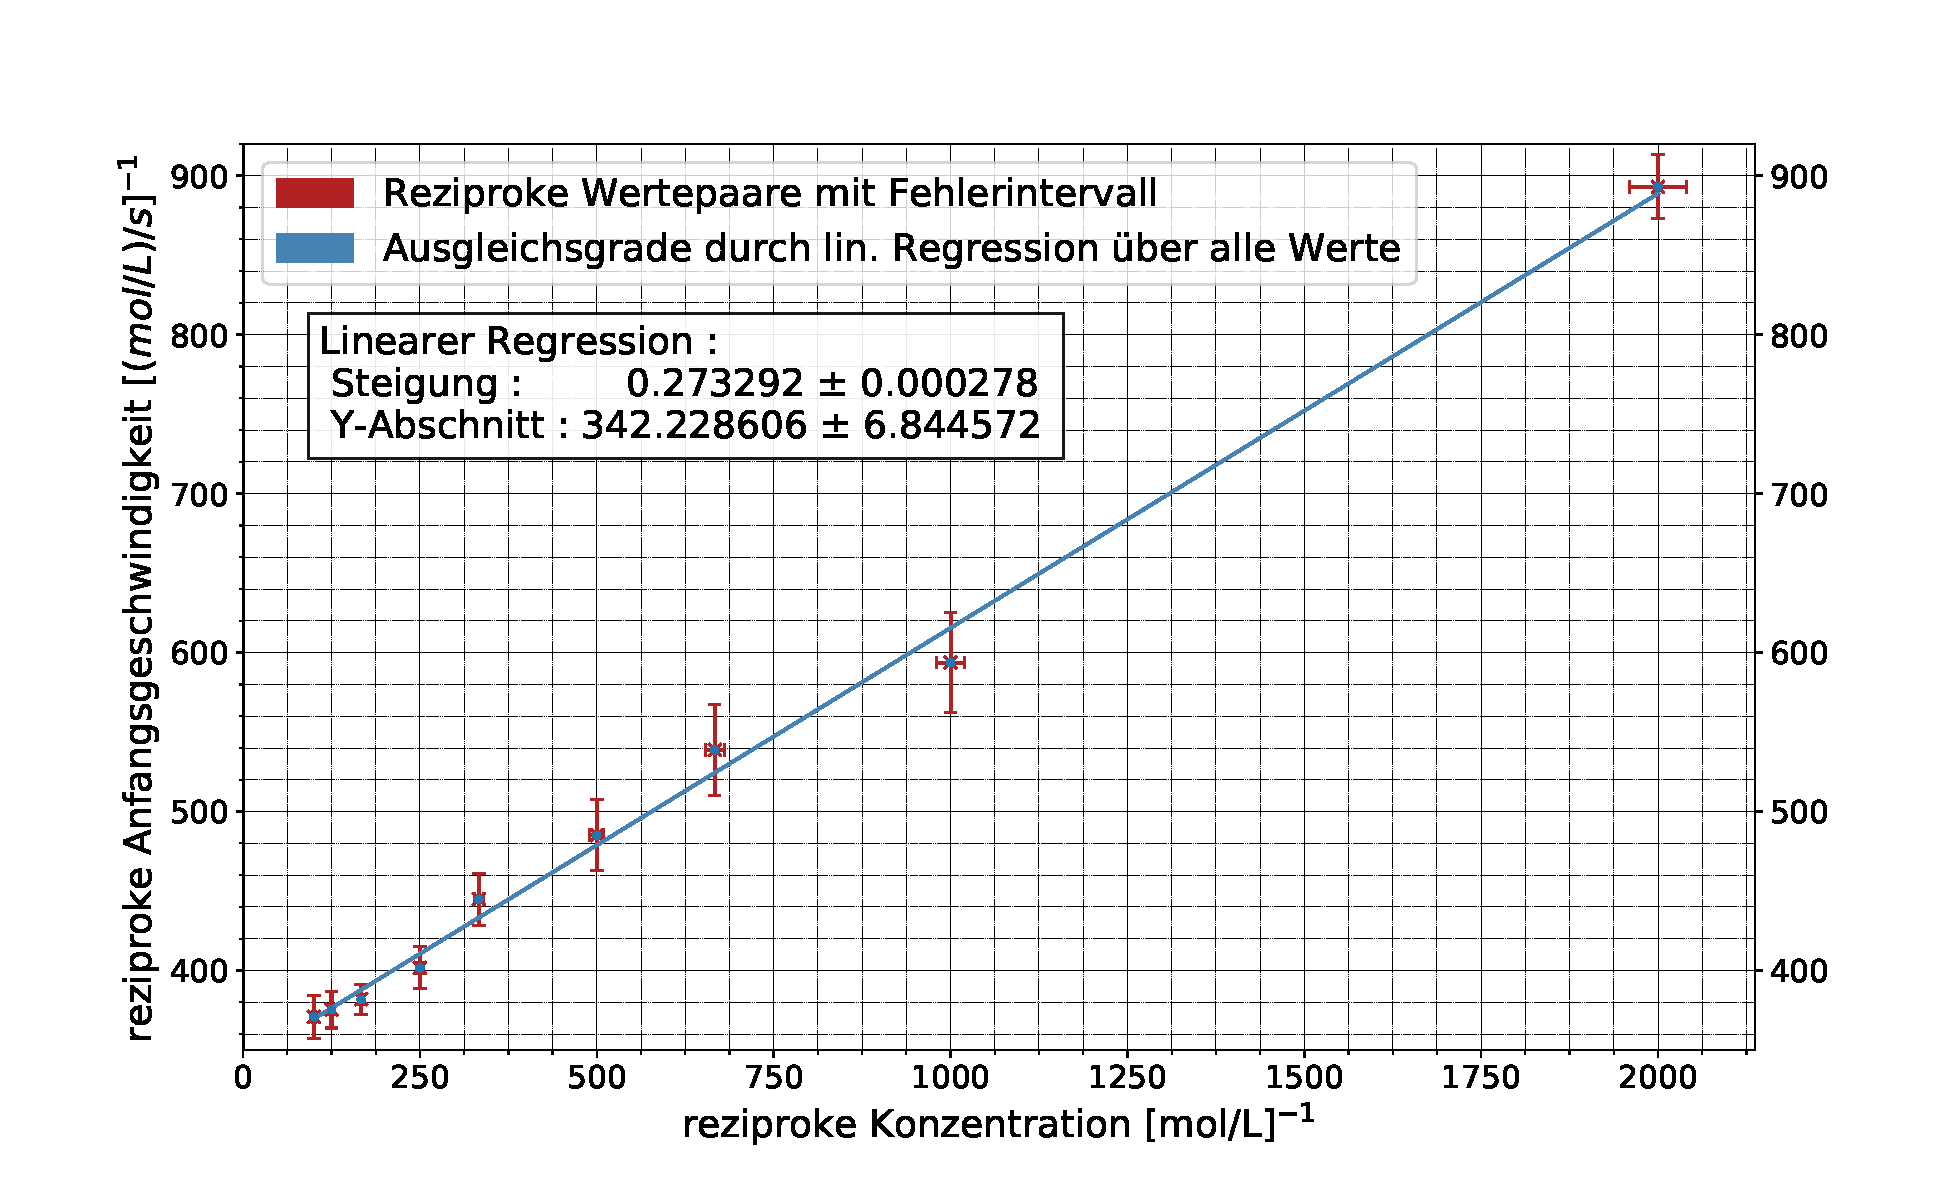
\includegraphics[width=\columnwidth]{Bilder/Lineweaver.pdf}
	\end{minipage}
	\caption{Auftragung der neun reziproken Wertepaare als Anfangsgeschwindigkeit über Konzentration. Die Fehler resultieren bezogen auf die Y-Achse aus den Fehlern der Steigungen und in der X-Achse aus der Messungenauigkeit von $2\%$. Die Ausgleichsgerade wurde durch eine lineare Regression über alle Punkte in der Programmiersprache \textit{python} erzeugt. Der Fehler bezieht sich neben dem Fehler des Verfahrens ebenfalls auf zuvor angesprochene fehlerbehaftete Größen.}
	\label{Lineweaver}
\end{figure}
Die Geradengleichung ergibt sich also in fehlerfreier Darstellung wie folgt : 
\begin{equation}
g(x) = 27.33x + 34222.86
\label{Geradengleichung}
\end{equation}
Gemäß Gleichung \ref{eq:lineweaverPlot} lässt sich hierdurch $\frac{1}{v_{max}}$ als Y-Achsenabschnitt (als $n$) sowie ferner $\frac{K_M}{v_{max}}$ als Steigung (als :$(m)$) bestimmen. Die Fehler resultieren aus den Fehlern der Regression.\\
\begin{equation}
v_{max} = \frac{1}{n} = \frac{1}{34222.86} \approx 2.92\cdot 10^{-5} \quad \left[\si{\frac{mol}{L\cdot s}}\right]
\end{equation}
\begin{equation}
\Delta v_{max} = |\frac{\partial v_{max}}{\partial n}|\Delta n = |-\frac{1}{n^2}|\Delta n \approx \pm 0.03  \cdot 10^{-5}\quad \left[\si{\frac{mol}{L\cdot s}}\right]
\end{equation}
Es ergibt sich somit : 
\begin{equation}
v_{max} = (2.92 \pm 0.03 )\cdot 10^{-5}  \quad \left[\si{\frac{mol}{L\cdot s}}\right]
\end{equation}\\
Die Michaelis Menten Konstante ergibt sich als Produkt der Steigung und des zuvor bestimmten $v_{max}$. Betrachte ferner für die Einheitenberechnung, dass die Steigung in $  [\si{s}]$, da $ [\si{\frac{mol}{L}\cdot \frac{L\cdot s}{mol} = s}]$: 
\begin{equation}
K_M = v_{max} \cdot m = 2.92 \cdot 10^{-5} \, \si{\frac{mol}{L\cdot s}}\,\, \cdot \,\,27.33  \,\si{s} \approx 7.98 \cdot 10^{-4} \, \left[\si{\frac{mol}{L}}\right]
\end{equation}\\
Der Fehler resultiert analog als Summe der partiellen Ableitungen gemäße : 
\begin{equation}
\Delta K_M = |\frac{\partial K_M}{\partial v_{max}}|\Delta v_{max} + |\frac{\partial K_M}{\partial m}|\Delta m  = m \Delta v_{max} + v_{max}\Delta m \approx 1.08 \cdot 10^{-5} \,\left[\si{\frac{mol}{L}}\right]
\end{equation}
Der Wert der Michaelis Menten Konstante ist also : 
\begin{equation}
K_M = (7.98 \pm 0.12) \cdot 10^{-4} \,\left[\si{\frac{mol}{L}}\right]
\end{equation}
Die Übergangskonstante $k_2$ kann unter Nutzung der Konzentration der verwendeten Urease bestimmt werden. Die molare Masse der Urease betrage $M[\text{Urease}] = 545 \, \si{g/mol} $. Es wurden $m = 0.105\,\si{g}$ der Urease abgewogen. Das Volumen ergibt sich nach der Verdünnung auf das elffache Volumen als $V=0.94\,\si{L}$. Die Konzentration der Urease wurde mit einer Messungenauigkeit von ungefähr $10\%$, basierend des Einwiegens sowie der Verdünnung angenommen. Es ergibt sich :
\begin{equation}
[Urease]_0 = \frac{m}{M}\cdot \frac{1}{V} =  (2.05 \pm 0.21)\cdot 10^{-7} \,\left[\si{\frac{mol}{L}}\right]
\end{equation} 
bestimmt. Im Anschluss ergibt sich $k_2$ als : 
\begin{equation}
k_2 = \frac{v_{max}}{[Urease]_0} = \frac{2.92\cdot 10^{-5}\, \si{\frac{mol}{L\cdot s}}}{2.05 \cdot 10^{-7} \, \si{\frac{mol}{L}}} \approx 142.5 \, \left[\si{\frac{1}{s}}\right]
\label{eq:k2}
\end{equation}
\\
Sowie dessen Fehler : 
\begin{equation}
\Delta k_2 = \left|\frac{\partial k_2}{\partial v_{max}}\right|\Delta v_{max} + \left|\frac{\partial k_2}{\partial [Urease]_0}\right|\Delta [Urease]_0  = ...
\end{equation}
\begin{equation*}
... \left|\frac{1}{v_{max}}\right| \Delta v_{max} + \left|\frac{v_{max}}{([Urease]_0)^2}\right|\Delta [Urease]_0 \approx 14.6 \,\left[\si{\frac{1}{s}}\right]
\end{equation*}
\\
Die Übergangskonstante $k_2$ lautet somit : 
\begin{equation}
k_2 = (142.5 \pm 14.6)\,\left[\si{\frac{1}{s}}\right]
\end{equation}
%\end{document}